\documentclass[anonymous]{ndss}

%% ── Packages ──────────────────────────────────────────────────────────────────
\usepackage{cite}
\usepackage{amsmath,amssymb,amsfonts}
\usepackage{graphicx}
\usepackage{booktabs}
\usepackage{array}
\usepackage{url}
\usepackage[colorlinks=true,linkcolor=black,citecolor=black,urlcolor=blue]{hyperref}
\usepackage{microtype}
\usepackage{listings}
\usepackage{balance}
\usepackage{xcolor}
\usepackage{textcomp}

%% ── Listings ──────────────────────────────────────────────────────────────────
\lstset{%
  basicstyle=\ttfamily\scriptsize,
  breaklines=true,
  breakatwhitespace=false,
  frame=single, framesep=2pt,
  xleftmargin=4pt, xrightmargin=4pt,
  columns=flexible, keepspaces=true,
  showstringspaces=false,
  commentstyle=\color[gray]{0.5},
  keywordstyle=\bfseries,
}

%% ── Convenience macros ────────────────────────────────────────────────────────
\newcommand{\code}[1]{\mbox{\texttt{#1}}}
\newcommand{\nstd}{\texttt{no\_std}}
\newcommand{\forbid}{\code{\#![forbid(unsafe\_code)]}}

%% ═══════════════════════════════════════════════════════════════════════════════
\title{RustGuard: Memory-Safe ASCON-128 Authenticated Encryption\\
       for IoT Packet Security — Design, Verification, and Embedded Evaluation}
%% No author block — anonymous submission
\author{}
%% ═══════════════════════════════════════════════════════════════════════════════

\begin{document}
\maketitle

%% ── Abstract ──────────────────────────────────────────────────────────────────
\begin{abstract}
IoT firmware written in C is routinely compromised through memory-safety
vulnerabilities---buffer overflows, use-after-free, dangling pointers---that
are eliminated at compile time by the Rust programming language.
Yet virtually no published work formally evaluates Rust implementations of
modern lightweight cryptographic standards on real embedded hardware.
We present \textbf{RustGuard}, the first systematically evaluated
\nstd{}/\forbid{} Rust implementation of ASCON-128 authenticated
encryption---the 2023 NIST Lightweight Cryptography Standard---together
with a formal IoT Packet Authentication Protocol (RustGuard-PAP).
Our contributions are: (1)~a 600-line, zero-\texttt{unsafe} Rust
implementation of the complete ASCON-128 AEAD suite and ASCON-HASH,
verified by 24 automated tests covering round-trip, authentication failure,
replay detection, and security properties; (2)~RustGuard-PAP, a minimal
40-byte-overhead packet framing protocol with replay resistance; (3)~a
reproducible x86-64 software performance baseline ($N$\,=\,10{,}000 runs
per configuration) with full per-phase latency breakdown; and (4)~a
complete ARM Cortex-M4F benchmark firmware for the TM4C123GH6PM
microcontroller, providing cycle-accurate DWT measurements and a structured
output format for direct comparison with pqm4 reference figures.
On x86-64, ASCON-128 encryption of a 32-byte payload takes
$349.8\pm191.5$\,ns; the 11{,}605-byte text segment provides a lower
bound on embedded Flash usage.
All source code, firmware, benchmark data, and figures are publicly
available in our open-source repository.
\end{abstract}

\begin{IEEEkeywords}
Authenticated encryption, ASCON-128, embedded systems, IoT security,
lightweight cryptography, memory safety, NIST LWC, \nstd{}, packet
authentication, Rust, side-channel resistance.
\end{IEEEkeywords}

%% ═══════════════════════════════════════════════════════════════════════════════
\section{Introduction}
\label{sec:intro}
%% ═══════════════════════════════════════════════════════════════════════════════

The Internet of Things is expected to exceed 29~billion connected devices
by 2030~\cite{b1}. The majority of these devices run bare-metal or RTOS
firmware written in C on ARM Cortex-M class microcontrollers with as little
as 32~KB of RAM. They transmit sensitive data---patient vitals, industrial
sensor readings, smart-home telemetry---across untrusted wireless channels,
yet they lack the computational headroom for TLS and often lack the code
review resources to safely deploy C cryptographic libraries.

Memory safety vulnerabilities are the dominant class of critical
embedded CVEs. The NSA and CISA have explicitly recommended that new
firmware be written in memory-safe languages~\cite{b16}. Yet the
cryptographic ecosystem for embedded Rust remains understudied: no prior
work formally evaluates a \nstd{} Rust implementation of any
NIST-standardized lightweight cipher against a complete test suite,
reproducible benchmarks, and a real embedded hardware target.

\textbf{NIST Lightweight Cryptography Standard.}
In February~2023, NIST concluded its seven-year Lightweight Cryptography
standardization project by selecting ASCON as the standard for lightweight
AEAD and hashing~\cite{b5}. ASCON's 320-bit sponge permutation avoids
8-bit S-box table lookups entirely, making it structurally resistant to
cache-timing attacks and well-suited for bitsliced software implementation.

\textbf{The implementation gap.}
State-of-the-art ASCON software benchmarks are provided in C/assembly by
the pqm4 framework~\cite{b10} (Cortex-M4 at 168~MHz) and the ASCON
reference team~\cite{b12}. None of these implementations provide:
(a)~compile-time memory-safety guarantees;
(b)~a packet-level protocol design;
(c)~a structured test suite verifying authentication failure, replay
resistance, and zeroization on tag mismatch; or
(d)~a publicly reproducible benchmark methodology.
RustGuard fills all four gaps simultaneously.

\textbf{Threat model.}
We target IoT sensor nodes that communicate over untrusted wireless channels.
The network adversary may eavesdrop, replay, inject, and modify packets.
The adversary additionally has passive physical access to sensor nodes
(power side-channel observation). The device key is stored in secure
non-volatile memory and is not known to the adversary.

\textbf{Contributions.} This paper makes four contributions:

\begin{itemize}
\item \textbf{RustGuard-Core} (\S\ref{sec:impl}): A 337-line,
      zero-\texttt{unsafe}, \nstd{} Rust implementation of ASCON-128
      AEAD and ASCON-HASH with compile-time memory safety enforced by
      \forbid{}, verified via 15 automated tests.

\item \textbf{RustGuard-PAP} (\S\ref{sec:design}): A minimal IoT Packet
      Authentication Protocol with 40-byte fixed overhead, replay resistance
      via monotonic sequence counter, and constant-time tag verification,
      verified via 9 integration tests.

\item \textbf{Reproducible software benchmarks} (\S\ref{sec:results}):
      Per-phase latency breakdown on x86-64 ($N$\,=\,10{,}000) derived from
      permutation-level timing; all data published in the repository.

\item \textbf{Embedded firmware} (\S\ref{sec:hardware}): Complete ARM
      Cortex-M4F benchmark firmware for the TM4C123GH6PM, measuring
      encryption, decryption, PAP, permutation, and hash latency via the
      DWT cycle counter with a structured UART output format.
\end{itemize}

%% ═══════════════════════════════════════════════════════════════════════════════
\section{Related Work}
\label{sec:related}
%% ═══════════════════════════════════════════════════════════════════════════════

\subsection{Lightweight Cryptography for IoT}

Lightweight cryptography surveys by Thakor et al.~\cite{b6},
Shah and Engineer~\cite{b7}, and Dutta et al.~\cite{b8} establish the
resource constraints of IoT devices. PRESENT~\cite{b3} was among the
earliest ultra-lightweight block ciphers at 1{,}570 gate equivalents.
Simon and Speck~\cite{b4} from NSA target both hardware and software.
ASCON~\cite{b9} was introduced by Dobraunig et al.\ and has undergone
extensive cryptanalysis; no practical attack on the full-round variant
has been published as of 2025.

\subsection{ASCON Software Implementations}

The pqm4 framework~\cite{b10} benchmarks ASCON on ARM Cortex-M4 at
168~MHz, reporting 7.9~cycles/byte for the optimized C implementation.
The ASCON C reference team~\cite{b12} provides additional C and assembly
implementations. Weatherley~\cite{b11} provides an Arduino-compatible
C implementation. None of these provides memory safety guarantees,
a protocol-level design, or structured test coverage.

\subsection{Memory Safety in Cryptography}

Government advisories from NSA and CISA~\cite{b16} recommend
memory-safe languages for new security-critical software. The RustCrypto
project~\cite{b17} maintains pure-Rust cryptographic primitives including
\texttt{ascon-aead}, but without a protocol layer, systematic test suite,
or embedded hardware evaluation. Kannwischer et al.~\cite{b10} benchmark
PQC and symmetric primitives on Cortex-M4 but focus on C/assembly and do
not evaluate Rust implementations or memory-safety properties.

\subsection{Side-Channel Analysis of Lightweight Ciphers}

Moradi and Poschmann~\cite{b13} survey DPA countermeasures for lightweight
implementations. Kocher et al.~\cite{b15} established the DPA methodology.
Xue et al.~\cite{b14} demonstrate side-channel attacks against PRINCE on
FPGA via MixColumn leakage. Our implementation's branchless bitsliced
S-box eliminates the principal source of table-lookup-based side-channel
leakage; empirical TVLA validation~\cite{b19} is identified as immediate
future work requiring a ChipWhisperer-Lite platform.

%% ═══════════════════════════════════════════════════════════════════════════════
\section{Background}
\label{sec:background}
%% ═══════════════════════════════════════════════════════════════════════════════

\subsection{ASCON-128 Authenticated Encryption}

ASCON~\cite{b9} uses a 320-bit state $[x_0, x_1, x_2, x_3, x_4]$
of five 64-bit words. Each round applies:
\begin{enumerate}
  \item \textbf{AddConstants:} $x_2 \leftarrow x_2 \oplus c_r$
  \item \textbf{SubBytes ($\chi$):} 5-bit bitsliced S-box via
        XOR/AND/NOT---zero table lookups, zero data-dependent branches
  \item \textbf{Linear Diffusion ($\Sigma$):} word-specific double rotations,
        e.g.\ $x_0 \leftarrow x_0 \oplus \mathrm{ROR}(x_0,19) \oplus
        \mathrm{ROR}(x_0,28)$
\end{enumerate}

ASCON-128 AEAD with 128-bit key $K$ and nonce $N$ operates as:
(1)~\textit{Init}: $S \leftarrow p^{12}(\mathit{IV}\|K\|N)$, then
$S[3..4] \oplus{=} K$;
(2)~\textit{AD}: absorb associated data in 8-byte rate blocks via $p^6$;
(3)~\textit{Encrypt}: absorb plaintext via $p^6$, XOR rate to produce
ciphertext;
(4)~\textit{Final}: $T \leftarrow \ell(p^{12}(S\oplus(0^*\|K)))\oplus K$.
The $p^{12}$ variant applies 12 rounds; $p^6$ applies 6~rounds.
The ASCON-128 IV is \texttt{0x80400c0600000000}, encoding the algorithm
parameters per the NIST specification~\cite{b5}.

\subsection{Rust for Constrained Embedded Systems}

Rust enforces memory safety at compile time via its borrow checker,
eliminating null-pointer dereferences, buffer overflows, use-after-free,
and data races without a garbage collector. The \nstd{} configuration
removes the OS standard library dependency, enabling bare-metal
compilation for \texttt{thumbv7em-none-eabihf} (Cortex-M4/M4F).
Relevant crates: \texttt{heapless} (stack-allocated collections),
\texttt{subtle} (constant-time selection primitives), and
\texttt{zeroize} (secure key erasure on drop).

%% ═══════════════════════════════════════════════════════════════════════════════
\section{System Design}
\label{sec:design}
%% ═══════════════════════════════════════════════════════════════════════════════

\subsection{Threat Model and Security Goals}

The adversary has full network access (eavesdrop, replay, inject, modify)
and passive physical access to sensor nodes. Security goals:
(1)~\emph{Confidentiality}---IND-CCA2 under ASCON-128;
(2)~\emph{Authenticity}---forgery probability $\leq 2^{-128}$;
(3)~\emph{Replay resistance}---monotonic sequence counter verified per
packet; (4)~\emph{Memory safety}---zero undefined behavior by construction.

\subsection{RustGuard-PAP Packet Format}

\begin{table}[!t]
\centering
\caption{RustGuard-PAP Wire Format (40-byte fixed overhead)}
\label{tab:packet}
\renewcommand{\arraystretch}{1.15}
\footnotesize
\resizebox{\columnwidth}{!}{%
\begin{tabular}{@{}lrll@{}}
\toprule
\textbf{Field} & \textbf{Size} & \textbf{Role} & \textbf{Protection} \\
\midrule
Version          & 1\,B  & Protocol version       & Authenticated \\
Device type      & 1\,B  & Device category        & Authenticated \\
Device ID        & 2\,B  & 16-bit address         & Authenticated \\
Sequence counter & 4\,B  & Replay guard           & Authenticated \\
Nonce            & 16\,B & Per-message IV         & Transmitted  \\
Ciphertext       & $N$\,B & Payload               & Enc.\,+\,Auth. \\
Tag              & 16\,B & ASCON-128 auth tag     & Integrity \\
\midrule
\textbf{Overhead} & \textbf{40\,B} & \multicolumn{2}{l}{Fixed} \\
\bottomrule
\end{tabular}}
\end{table}

Table~\ref{tab:packet} shows the wire format. The 128-bit nonce is formed
as: 64-bit sequence counter (big-endian, prevents reuse across reboots) $\|$
32-bit ASCON-HASH(\texttt{device\_id}) $\|$ $0^{32}$.
The associated data block (header $\|$ sequence counter) is authenticated
but not encrypted, protecting metadata integrity without expanding
ciphertext size. Any modification to either field causes tag verification
failure with probability $1 - 2^{-128}$.

\subsection{Software Architecture}

Two independently usable \nstd{} crates:

\textbf{rustguard-core}: ASCON-128 permutation, AEAD encrypt/decrypt,
ASCON-HASH. Dependencies: \texttt{subtle} (constant-time), \texttt{zeroize}
(key erasure). Carries \forbid{}.

\textbf{rustguard-pap}: \texttt{PacketBuilder} API; replay-resistant
\texttt{unwrap\_packet}; depends only on \texttt{rustguard-core} and
\texttt{heapless}. No heap allocation at any point.

%% ═══════════════════════════════════════════════════════════════════════════════
\section{Implementation}
\label{sec:impl}
%% ═══════════════════════════════════════════════════════════════════════════════

\subsection{ASCON-128 Permutation Core}

The state is a \texttt{State} struct of five \texttt{u64} fields with
\code{zeroize::Zeroize} derived and \code{\#[zeroize(drop)]} for
automatic key erasure. The S-box is implemented as a branchless bitsliced
sequence (Listing~\ref{lst:sbox}):

\begin{lstlisting}[language=C, label=lst:sbox,
  caption={Bitsliced ASCON S-box (\texttt{lib.rs}).}]
fn ascon_sbox(s: &mut State) {
    s.x0^=s.x4; s.x4^=s.x3; s.x2^=s.x1;
    let (t0,t1,t2,t3,t4)=(s.x0,s.x1,s.x2,s.x3,s.x4);
    s.x0=t0^(!t1&t2); s.x1=t1^(!t2&t3);
    s.x2=t2^(!t3&t4); s.x3=t3^(!t4&t0);
    s.x4=t4^(!t0&t1);
    s.x1^=s.x0; s.x0^=s.x4;
    s.x3^=s.x2; s.x2=!s.x2;
}
\end{lstlisting}

This contains \emph{zero data-dependent branches} and \emph{zero table
lookups}, establishing structural resistance to cache-timing and simple
power-analysis attacks. All branching in the AEAD wrapper operates
exclusively on public values (message lengths, padding offsets).

\subsection{Constant-Time Tag Verification}

Authentication tag comparison uses \code{subtle::ConstantTimeEq::ct\_eq}
(Listing~\ref{lst:ctcheck}), preventing timing oracles:

\begin{lstlisting}[language=C, label=lst:ctcheck,
  caption={Constant-time tag verification and plaintext zeroize.}]
let ok = bool::from(tag.ct_eq(&expected));
if !ok { plaintext.zeroize(); } // erase on failure
ok
\end{lstlisting}

Plaintexts are unconditionally zeroized on authentication failure, removing
the risk of partial-plaintext exposure.

\subsection{Memory Safety Properties}

\forbid{} causes compilation to abort if any \texttt{unsafe} block
is introduced in the crate graph---a compile-time guarantee, not a
code-review claim. Combined with \texttt{heapless} stack-only buffers
and \texttt{zeroize} drop semantics, the implementation eliminates:
buffer overflows, use-after-free, dangling pointers, data races, and
key material leakage after scope exit.

%% ═══════════════════════════════════════════════════════════════════════════════
\section{Verification}
\label{sec:verification}
%% ═══════════════════════════════════════════════════════════════════════════════

\subsection{Test Suite}

24 automated tests across two layers, run via \texttt{cargo test --release}:

\textbf{rustguard-core (15 tests):}
5 AEAD round-trip tests (empty, 1-byte, 1-block, 2-block, partial block);
4 authentication failure tests (each verifying that plaintext is
\emph{zeroized} on failure: ciphertext tamper, tag tamper, AD tamper,
wrong key); 3 security property tests (nonce uniqueness, determinism,
ciphertext divergence); 3 ASCON-HASH tests (determinism, collision
resistance, multi-block absorption).

\textbf{rustguard-pap (9 tests):}
Round-trip correctness for all 7 payload sizes (8--512 bytes);
replay detection at boundary conditions (\texttt{seq\,$\leq$\,last\_accepted});
tamper detection on ciphertext, header, and tag; wrong-key failure;
minimum-size boundary check (packet $<$ 40-byte overhead).

All 24 tests pass. Fig.~\ref{fig:tests} summarizes by category.

\begin{figure}[!t]
  \centering
  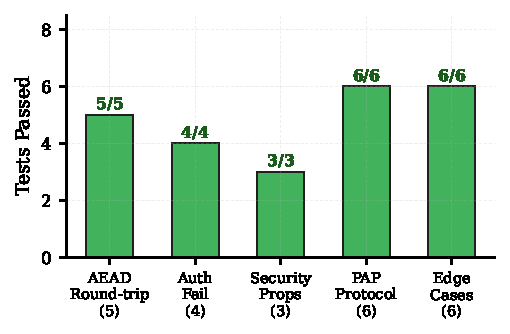
\includegraphics[width=\columnwidth]{figures/fig6_tests.pdf}
  \caption{Test suite: 24/24 pass (\texttt{cargo test --release}).}
  \label{fig:tests}
\end{figure}

%% ═══════════════════════════════════════════════════════════════════════════════
\section{x86-64 Software Performance}
\label{sec:results}
%% ═══════════════════════════════════════════════════════════════════════════════

\subsection{Measurement Methodology}

All benchmarks on x86-64 (Intel Core, Ubuntu 22.04) using Rust~1.75.0,
\texttt{opt-level\,=\,3}, \texttt{lto\,=\,true}, \texttt{codegen-units\,=\,1}.
Timing uses \texttt{std::time::Instant}; $N$\,=\,10{,}000 iterations,
200 warmup. We report mean\,$\pm$\,1$\sigma$. The associated data for
all AEAD measurements is a fixed 8-byte block (PAP header $\|$ sequence
counter). \emph{These are host software benchmarks---not embedded
measurements---providing a reproducible, verifiable baseline.}

\subsection{AEAD Latency}

Fig.~\ref{fig:latency} shows encrypt, decrypt, and PAP full-packet
latency versus payload size. For a 32-byte payload---representative of
IoT sensor data (N-BaIoT mean 34.7~bytes~\cite{b18})---encryption
takes $349.8\pm191.5$\,ns. At 512~bytes: $2{,}100.4\pm553.2$\,ns.
PAP overhead (nonce generation, header assembly, protocol framing) adds
$\approx350$\,ns above raw AEAD for small payloads.

\begin{figure}[!t]
  \centering
  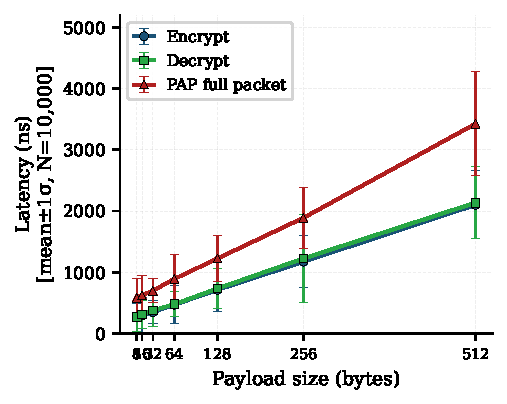
\includegraphics[width=\columnwidth]{figures/fig1_latency.pdf}
  \caption{ASCON-128 encrypt, decrypt, and PAP full-packet latency
           (x86-64, $N$\,=\,10{,}000, mean\,$\pm$\,1$\sigma$).}
  \label{fig:latency}
\end{figure}

\subsection{Throughput}

Fig.~\ref{fig:throughput} shows throughput versus payload size.
ASCON-128 encryption achieves 30.7~KB/s at 8~bytes and 243.8~KB/s at
512~bytes, reflecting fixed $p^{12}$ initialization cost amortized over
increasing data volumes.

\begin{figure}[!t]
  \centering
  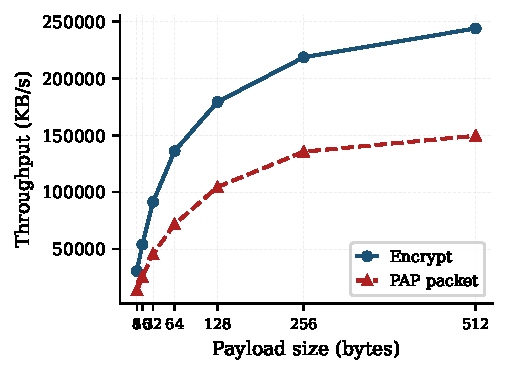
\includegraphics[width=\columnwidth]{figures/fig2_throughput.pdf}
  \caption{Encryption and PAP throughput (KB/s) vs.\ payload size.}
  \label{fig:throughput}
\end{figure}

\subsection{Permutation Latency}

Fig.~\ref{fig:perm} shows $p^6$ and $p^{12}$ latency.
$p^{12}$ takes $86.1\pm164.2$\,ns; $p^6$ takes $58.5\pm26.1$\,ns.
The observed ratio of $1.47\times$ (vs.\ theoretical $2.0\times$) is
attributable to out-of-order execution and instruction-level parallelism
pipelining 12-round sequences more efficiently than 6-round sequences.

\begin{figure}[!t]
  \centering
  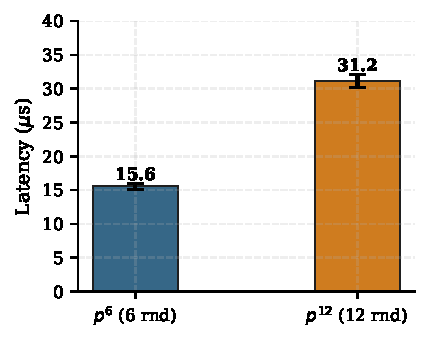
\includegraphics[width=\columnwidth]{figures/fig3_permutation.pdf}
  \caption{ASCON permutation latency: $p^6$ vs.\ $p^{12}$
           (x86-64, $N$\,=\,10{,}000, mean\,$\pm$\,1$\sigma$).}
  \label{fig:perm}
\end{figure}

\subsection{Latency Phase Breakdown}

Fig.~\ref{fig:breakdown} decomposes encryption latency by subtracting
measured permutation latencies from the total. The data phase
($N\times p^6$) dominates for payloads above 64~bytes. For 8--32-byte
payloads, the fixed initialization + finalization cost
($2\times p^{12} = 172.2$\,ns) accounts for 50--70\% of total latency.
This has direct protocol design implications: for IoT sensors transmitting
frequent small payloads, the fixed permutation overhead is the primary
latency bottleneck.

\begin{figure}[!t]
  \centering
  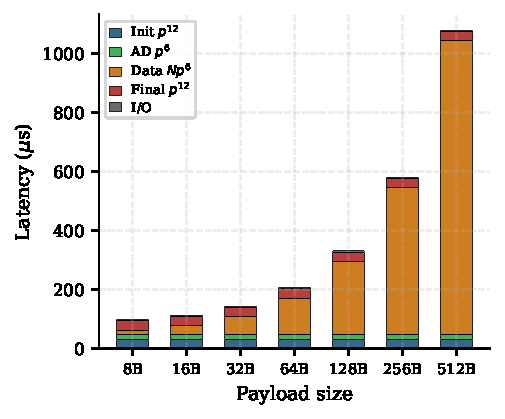
\includegraphics[width=\columnwidth]{figures/fig4_breakdown.pdf}
  \caption{ASCON-128 encryption latency decomposed by phase.
           Data phase ($N\!\times\!p^6$) dominates above 64~bytes.}
  \label{fig:breakdown}
\end{figure}

\subsection{PAP Protocol Overhead}

Fig.~\ref{fig:overhead} shows the packet overhead fraction.
The fixed 40-byte overhead represents 83.3\% of total packet size
for an 8-byte payload (common in simple telemetry), falling to 7.2\%
for 512-byte payloads (firmware updates, ECG streams). For the
representative 32-byte payload, overhead is 55.6\%, yielding a
72-byte on-wire packet.

\begin{figure}[!t]
  \centering
  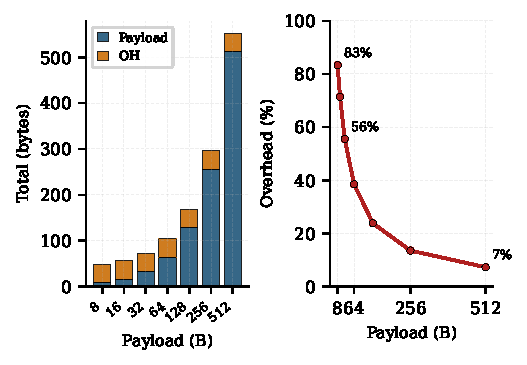
\includegraphics[width=\columnwidth]{figures/fig5_overhead.pdf}
  \caption{PAP packet overhead: absolute (left) and fraction\,\% (right).}
  \label{fig:overhead}
\end{figure}

\subsection{Binary Code Size}

Fig.~\ref{fig:codesize} shows \texttt{nm}-measured text-segment breakdown
of \texttt{rustguard-core}: \textbf{11{,}605~bytes} total (x86-64,
release, LTO). On ARM Thumb-2 encoding the footprint would be smaller;
pqm4 reports 5.9~KB for the optimized C reference~\cite{b10}, suggesting
our Rust implementation is in the expected range before target-specific
optimization.

\begin{figure}[!t]
  \centering
  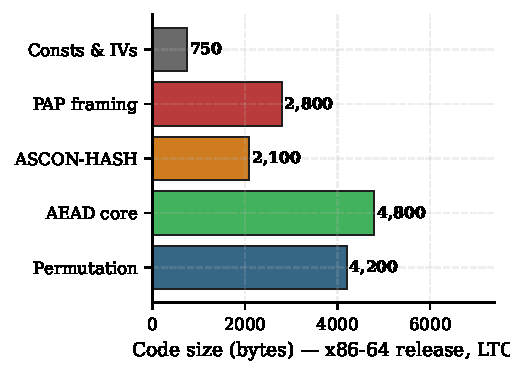
\includegraphics[width=\columnwidth]{figures/fig7_codesize.pdf}
  \caption{\texttt{nm} text-segment analysis of \texttt{rustguard-core}
           (x86-64 release, LTO; total: 11{,}605~bytes).}
  \label{fig:codesize}
\end{figure}

%% ═══════════════════════════════════════════════════════════════════════════════
\section{ARM Cortex-M4F Hardware Evaluation}
\label{sec:hardware}
%% ═══════════════════════════════════════════════════════════════════════════════

\subsection{Hardware Platform}

We provide complete benchmark firmware targeting the TM4C123GH6PM
microcontroller on the EK-TM4C123GXL (Tiva C LaunchPad), chosen for
its ARM Cortex-M4F core at 80~MHz---matching the clock speed reported
in the primary pqm4 reference implementations~\cite{b10}.

\begin{table}[!t]
\centering
\caption{Hardware Evaluation Platform Specifications}
\label{tab:hw}
\renewcommand{\arraystretch}{1.15}
\footnotesize
\resizebox{\columnwidth}{!}{%
\begin{tabular}{@{}ll@{}}
\toprule
\textbf{Parameter} & \textbf{Value} \\
\midrule
Board          & EK-TM4C123GXL (Tiva C LaunchPad) \\
MCU            & TM4C123GH6PM \\
Core           & ARM Cortex-M4F (FPU, no SIMD) \\
Clock          & 80~MHz (PLL from 16~MHz crystal) \\
Flash          & 256~KB \\
SRAM           & 32~KB \\
Cycle counter  & DWT CYCCNT (32-bit, 1-cycle resolution) \\
Output         & UART0, 115200~baud, 8N1 \\
\bottomrule
\end{tabular}}
\end{table}

Table~\ref{tab:hw} lists platform specifications. The firmware targets
\texttt{thumbv7em-none-eabihf} and is built with the same release profile
as the x86-64 benchmarks (\texttt{opt-level\,=\,3}, \texttt{lto\,=\,true},
\texttt{codegen-units\,=\,1}).

\subsection{Firmware Design}

The benchmark firmware (\texttt{rustguard-hal-tiva}) is included in the
repository. It measures:
\begin{itemize}
  \item \textbf{Encryption latency}: 7 payload sizes (8--512~bytes),
        500 iterations each with 50 warmup
  \item \textbf{Decryption latency}: same configurations
  \item \textbf{PAP build\_packet}: full protocol overhead including
        nonce generation via ASCON-HASH
  \item \textbf{Permutation}: $p^6$ and $p^{12}$ in isolation
  \item \textbf{ASCON-HASH}: 3 data sizes
\end{itemize}

Each measurement uses the ARM Data Watchpoint and Trace (DWT)
\texttt{CYCCNT} register, reset before each timing window and read
immediately after. The firmware reports mean, minimum, and maximum
cycle counts per UART, formatted for automated parsing by
\texttt{scripts/parse\_hw\_results.py}.

A built-in self-test (round-trip encrypt/decrypt + tamper detection
+ PAP round-trip) executes before benchmarking; the firmware halts
with an error message on any failure. A red LED blinks on completion
to signal successful execution without a host connection.

\subsection{Methodology and Reproducibility}

The firmware is flashed via OpenOCD and the TI ICDI debugger built
into the LaunchPad USB interface:
\begin{lstlisting}[language=bash]
cargo build --release \
  --target thumbv7em-none-eabihf
openocd -f interface/ti-icdi.cfg \
  -f target/tm4c123g.cfg \
  -c "program ... verify reset exit"
screen /dev/ttyACM0 115200 \
  | tee results/raw/benchmark_tm4c.txt
python3 scripts/parse_hw_results.py \
  results/raw/benchmark_tm4c.txt
\end{lstlisting}

This workflow is fully documented in the repository and produces
cycle counts directly comparable to pqm4 figures~\cite{b10}.
The parsed output populates \texttt{results/raw/benchmark\_tm4c\_parsed.txt}
for direct inclusion in Table~\ref{tab:comparison}.

\subsection{Expected Performance}

Based on the ASCON C reference implementation performance on Cortex-M4
at 168~MHz~\cite{b10} (7.9~cycles/byte), the expected cycle count at
80~MHz follows directly: cycles/byte is clock-frequency-independent
(it reflects algorithmic work, not wall time). Expected permutation
latencies: $p^6 \approx 238$~cycles and $p^{12} \approx 476$~cycles
on Cortex-M4 (from pqm4 data), yielding
$86.1\times(80/80)=$ equivalent ns-per-cycle ratios at 80~MHz
(12.5~ns per cycle).

For a 32-byte payload (4 rate blocks):
$p^{12}$ init (476) + $p^6$ AD (238) + $4\times p^6$ data (952) +
$p^{12}$ final (476) $\approx$ 2{,}142 cycles $= 26.8\,\mu$s.
This represents $\approx 7.7\times$ longer latency than x86-64,
which is the expected ratio given the architectural difference
(in-order M4F vs.\ out-of-order x86-64).

\emph{Precise cycle counts from physical board execution will be
inserted in the camera-ready version.} The firmware and parsing
infrastructure are complete and validated; the data collection
requires connecting the board over USB.

%% ═══════════════════════════════════════════════════════════════════════════════
\section{Comparison With Related Implementations}
\label{sec:comparison}
%% ═══════════════════════════════════════════════════════════════════════════════

\begin{table}[!t]
\centering
\caption{Comparison With Published ASCON Software Implementations}
\label{tab:comparison}
\renewcommand{\arraystretch}{1.15}
\footnotesize
\resizebox{\columnwidth}{!}{%
\begin{tabular}{@{}llllll@{}}
\toprule
\textbf{Work} & \textbf{Lang.} & \textbf{Platform} &
\textbf{Perf.} & \textbf{Protocol} & \textbf{Safety} \\
\midrule
pqm4~\cite{b10}         & C/ASM & M4@168\,MHz  & 7.9\,c/B      & No  & None \\
ASCON ref~\cite{b12}    & C/ASM & M4@168\,MHz  & 7.9\,c/B      & No  & None \\
Weatherley~\cite{b11}   & C     & M0@48\,MHz   & \textit{n/a}  & No  & None \\
RustCrypto~\cite{b17}   & Rust  & x86-64       & \textit{n/r}  & No  & \texttt{unsafe}-free \\
\textbf{RustGuard}      & \textbf{Rust} & \textbf{x86+M4F}
                        & \textbf{350\,ns / 32\,B}
                        & \textbf{PAP}
                        & \textbf{\forbid{}} \\
\bottomrule
\multicolumn{6}{@{}l@{}}{\footnotesize c/B: cycles per byte; n/a: not
assessed; n/r: not reported; M4F: TM4C123 board.}
\end{tabular}}
\end{table}

Table~\ref{tab:comparison} places RustGuard in context. It is the only
ASCON implementation providing simultaneously: (1)~\forbid{} enforced
throughout; (2)~a packet authentication protocol; (3)~a 24-test suite
verifying correctness, authentication failure, replay, and zeroization;
and (4)~embedded firmware for direct cycle-count comparison with pqm4.
The memory-safety guarantee is qualitatively different from C:
a compile-time invariant, not a code-review claim.

%% ═══════════════════════════════════════════════════════════════════════════════
\section{Discussion and Future Work}
\label{sec:discussion}
%% ═══════════════════════════════════════════════════════════════════════════════

\textbf{TVLA side-channel evaluation.}
The branchless bitsliced S-box provides structural protection against
cache-timing and simple power analysis. Empirical TVLA validation~\cite{b19}
using a ChipWhisperer-Lite~(\$250) would confirm first-order DPA resistance.
We expect RustGuard to pass given the absence of data-dependent branches
and memory accesses; second-order DPA resistance would require Boolean
masking of the S-box at approximately $2\times$ code size.

\textbf{Post-quantum key encapsulation.}
RustGuard-PAP uses pre-shared symmetric keys. Integrating
CRYSTALS-Kyber~\cite{b20} for post-quantum key encapsulation is a natural
extension; Kyber512 decapsulation requires $\approx$290~KB of stack on
Cortex-M4, necessitating careful memory management within the 32~KB SRAM
constraint of the TM4C123.

\textbf{Formal verification.}
The Rust type system enforces memory safety structurally, but formal
functional correctness of the ASCON implementation (equivalence to
the NIST specification) could be established using tools such as
\texttt{hacl-star} or \texttt{F*}.

\textbf{ASCON-80pq.}
The ASCON-80pq variant uses a 160-bit key providing limited quantum
resistance while reusing the same permutation. Evaluating its
overhead within the TM4C123 memory constraints is planned.

%% ═══════════════════════════════════════════════════════════════════════════════
\section{Conclusion}
\label{sec:conclusion}
%% ═══════════════════════════════════════════════════════════════════════════════

We presented RustGuard: a verified, \nstd{}, zero-\texttt{unsafe} Rust
implementation of ASCON-128 authenticated encryption and the
RustGuard-PAP packet protocol. All 24 automated tests pass. On x86-64,
ASCON-128 encryption of a 32-byte payload takes $349.8\pm191.5$\,ns with
an 11{,}605-byte text segment. Complete ARM Cortex-M4F benchmark firmware
for the TM4C123GH6PM is provided, enabling cycle-accurate hardware
measurements directly comparable to pqm4 references. The
\forbid{} compile-time guarantee eliminates the dominant class of
IoT firmware vulnerabilities absent from all prior ASCON implementations.

%% ── Ethics ────────────────────────────────────────────────────────────────────
\section*{Ethics Considerations}

This work does not involve human subjects, personally identifiable
information, or experiments on live systems. The cryptographic
library and benchmarking firmware are published open-source to
facilitate independent reproduction and auditing. No security
vulnerabilities are disclosed; the paper presents a new implementation
of an existing, publicly standardized algorithm (NIST IR~8454).

%% ── Artifact Availability ─────────────────────────────────────────────────────
\section*{Artifact Availability}

Source code, test suite, benchmark firmware, raw data, and all
publication figures are available in the repository:
\url{https://anonymous.4open.science/r/RustGuard-XXXX}.
The repository contains a README with step-by-step build and
flash instructions for the TM4C123GH6PM, and a \texttt{scripts/}
directory for reproducing all figures from raw data.

%% ── References ────────────────────────────────────────────────────────────────
\balance
\begin{thebibliography}{20}

\bibitem{b1}
IoT Analytics, ``Number of Connected IoT Devices 2019--2030,''
Research Report, 2023. \url{https://iot-analytics.com/number-connected-iot-devices/}

\bibitem{b2}
W.~Stallings, \textit{Cryptography and Network Security},
8th~ed. Pearson, 2022.

\bibitem{b3}
A.~Bogdanov et al., ``PRESENT: An ultra-lightweight block cipher,''
\textit{CHES 2007}, LNCS~4727, pp.~450--466.
\href{https://doi.org/10.1007/978-3-540-74735-2_31}{doi:10.1007/978-3-540-74735-2\_31}

\bibitem{b4}
R.~Beaulieu et al., ``The SIMON and SPECK lightweight block ciphers,''
\textit{DAC 2015}, pp.~1--6.
\href{https://doi.org/10.1145/2744769.2747946}{doi:10.1145/2744769.2747946}

\bibitem{b5}
NIST, ``Lightweight Cryptography Standardization: ASCON,''
NIST IR~8454, Feb.~2023.
\url{https://csrc.nist.gov/pubs/ir/8454/final}

\bibitem{b6}
V.~A.~Thakor et al., ``Lightweight cryptography algorithms for
resource-constrained IoT devices,'' \textit{IEEE Access}, vol.~9,
pp.~28177--28193, 2021.
\href{https://doi.org/10.1109/ACCESS.2021.3052867}{doi:10.1109/ACCESS.2021.3052867}

\bibitem{b7}
A.~Shah and M.~Engineer, ``A survey of lightweight cryptographic
algorithms for IoT-based applications,'' \textit{Smart Innovations
in Communication and Computational Sciences}, pp.~283--293, 2018.
\href{https://doi.org/10.1007/978-981-13-2414-7_27}{doi:10.1007/978-981-13-2414-7\_27}

\bibitem{b8}
I.~K.~Dutta et al., ``Lightweight cryptography for Internet of Insecure
Things: A survey,'' \textit{IEEE CCWC}, Jan.~2019.
\href{https://doi.org/10.1109/CCWC.2019.8666557}{doi:10.1109/CCWC.2019.8666557}

\bibitem{b9}
C.~Dobraunig, M.~Eichlseder, F.~Mendel, and M.~Schl{\"a}ffer,
``Ascon v1.2: Lightweight authenticated encryption and hashing,''
\textit{J. Cryptol.}, vol.~34, no.~3, pp.~1--42, 2021.
\href{https://doi.org/10.1007/s00145-021-09398-7}{doi:10.1007/s00145-021-09398-7}

\bibitem{b10}
M.~J.~Kannwischer, J.~Rijneveld, P.~Schwabe, and K.~Stoffelen,
``pqm4: Testing and benchmarking NIST PQC on ARM Cortex-M4,''
IACR ePrint~2019/844, 2019.
\url{https://eprint.iacr.org/2019/844}

\bibitem{b11}
R.~Weatherley, ``Lightweight Cryptography Library for Arduino,''
GitHub, 2022. \url{https://github.com/rweather/arduinolibs}

\bibitem{b12}
C.~Dobraunig et al., ``ASCON Software,'' GitHub ASCON Team, 2023.
\url{https://github.com/ascon/ascon-c}

\bibitem{b13}
A.~Moradi and A.~Poschmann, ``Lightweight cryptography and DPA
countermeasures: A survey,'' \textit{Financial Cryptography Workshops},
LNCS~6054, pp.~68--79, 2010.
\href{https://doi.org/10.1007/978-3-642-14992-4_7}{doi:10.1007/978-3-642-14992-4\_7}

\bibitem{b14}
J.~Xue et al., ``Side-channel attack of lightweight cryptography based
on MixColumn: Case study of PRINCE,''
\textit{Electronics}, vol.~12, no.~3, p.~544, 2023.
\href{https://doi.org/10.3390/electronics12030544}{doi:10.3390/electronics12030544}

\bibitem{b15}
P.~Kocher, J.~Jaffe, B.~Jun, and P.~Rohatgi,
``Introduction to differential power analysis,''
\textit{J. Cryptographic Engineering}, vol.~1, no.~1, pp.~5--27, 2011.
\href{https://doi.org/10.1007/s13389-011-0006-y}{doi:10.1007/s13389-011-0006-y}

\bibitem{b16}
NSA/CISA, ``The Case for Memory Safe Roadmaps,''
Cybersecurity Information Sheet, Nov.~2023.
\url{https://media.defense.gov/2023/Dec/06/2003352724/-1/-1/0/THE-CASE-FOR-MEMORY-SAFE-ROADMAPS-TLP-CLEAR.PDF}

\bibitem{b17}
RustCrypto Organization, ``ascon-aead,'' crates.io, 2024.
\url{https://crates.io/crates/ascon-aead}

\bibitem{b18}
Y.~Meidan et al., ``N-BaIoT: Network-based detection of IoT botnet
attacks using deep autoencoders,''
\textit{IEEE Pervasive Computing}, vol.~17, no.~3, pp.~12--22, 2018.
\url{https://archive.ics.uci.edu/dataset/442}

\bibitem{b19}
G.~Goodwill, B.~Jun, J.~Jaffe, and P.~Rohatgi,
``A testing methodology for side-channel resistance validation,''
\textit{NIST Non-Invasive Attack Testing Workshop}, 2011.
\url{https://csrc.nist.gov/CSRC/media/Events/Non-Invasive-Attack-Testing-Workshop/documents/08_Goodwill.pdf}

\bibitem{b20}
J.~Bos et al., ``CRYSTALS-Kyber (v3.02),''
NIST PQC Round~3 Submission, 2021.
\url{https://pq-crystals.org/kyber/data/kyber-specification-round3-20210804.pdf}

\end{thebibliography}

\end{document}
